\documentclass[conference]{IEEEtran}
%\IEEEoverridecommandlockouts
% The preceding line is only needed to identify funding in the first footnote. If that is unneeded, please comment it out.
\usepackage{cite}
\usepackage{amsmath,amssymb,amsfonts}
\usepackage{algorithmic}
\usepackage{graphicx}
\usepackage{textcomp}
\usepackage{xcolor}
\usepackage{booktabs}                        % AAB inserido
\usepackage[utf8]{inputenc}                  % AAB inserido
\usepackage{rotating}                        % AAB inserido
%\usepackage{subfigure}                       % AAB inserido
%\usepackage[export]{adjustbox}               % AAB inserido
\usepackage{bbm}

\ifCLASSOPTIONcompsoc                        % AAB inserido
\usepackage[caption=false,font=normalsize,labelfont=sf,textfont=sf]{subfig}
\else
\usepackage[caption=false,font=footnotesize]{subfig}
\fi
%\usepackage[round,sort,nonamebreak]{natbib}  % AAB inserido
%\usepackage[round,sort,nonamebreak]{natbib} % citação bibliográfica textual
\def\BibTeX{{\rm B\kern-.05em{\sc i\kern-.025em b}\kern-.08em
    T\kern-.1667em\lower.7ex\hbox{E}\kern-.125emX}}
%AAB
\DeclareMathOperator{\traco}{tr}
\graphicspath{{../../Dissertacao/figuras/}}
\begin{document}

\title{Fusion of Evidences for Edge Detection in PolSAR Images\\
%{\footnotesize \textsuperscript{*}Note: Sub-titles are not captured in Xplore and
%should not be used}
\thanks{Grantee Capes/PROSUP/Mackenzie.}
}

\author{\IEEEauthorblockN{Anderson A. de Borba}
\IEEEauthorblockA{\textit{Dept.\ Engenharia Elétrica e Computação} \\
\textit{UPM -- Universidade Presbiteriana Mackenzie}\\
IBMEC-SP\\
São Paulo, Brazil \\
anderson.borba@ibmec.edu.br}
\and
\IEEEauthorblockN{Maurício Marengoni}
\IEEEauthorblockA{\textit{Dept.\ Engenharia Elétrica e Computação} \\
\textit{UPM -- Universidade Presbiteriana Mackenzie}\\
São Paulo, Brazil \\
mauricio.marengoni@mackenzie.br}
\and
\IEEEauthorblockN{\hspace{6cm} Alejandro C. Frery}
\IEEEauthorblockA{\textit{\hspace{6cm}Laboratório de Computação Científica e Análise Numérica -- LACCAN} \\
\hspace{6cm}\textit{UFAL -- Universidade Federal de Alagoas}\\
\hspace{6cm} Maceió, Brazil \\
\hspace{6cm}acfrery@gmail.com}
}

\maketitle

\begin{abstract}
Polarimetric Synthetic Aperture Radar (PolSAR) has achieved an important position as a remote sensing imaging method. 
However, PolSAR images are contaminated with speckle, making its processing and analysis challenging tasks. 
The present study discusses an detection method based on the fusion of evidences obtained in the intensities channels of multilook PolSAR images.
The method consists of detecting transition points in the finest strip of data which spans two regions using the maximum likelihood.
This is applied to each of the three intensity channels (hh), (hv) and (vv). 
The fusion methods are simple average, stationary wavelet transform (SWT), principal component analysis (PCA) and ROC statistics.  
%%% Esperar o artigo ficar pronto e pontuar o que foi feito
The results indicate a good performance of the approach in detecting edges with possible paths for future research.
\end{abstract}

\begin{IEEEkeywords}
PolSAR, edge detection, maximum likelihood estimation, fusion
\end{IEEEkeywords}

\section{Introduction}\label{sec_01}

We present results on the detection and fusion of edge evidence applied to Polarimetric Synthetic Aperture Radar images (PolSAR). 
We employ models and algorithms as required for an appropriate treatment of their special statistical characteristics~\cite{slf_2008}.

Among the available edge detection techniques for SAR imagery, it is worth mentioning those based on the gradient~\cite{tlb, obw, flmc, fyf}, and on Markov chains~\cite{bf}.
The former suffer from the effect of speckle, and the latter lead to computer intensive methods.
Ref.~\cite{gfn} presents a comparison between several edge detectors. 

Alternatively, techniques based on statistical modeling have been used in edge detection~\cite{gmbf, fbgm, horrit, gfn} and, more recently, by means of \textit{Deep Learning}~\cite{bac, ztmxzxf, tabmm, xstz}.

This work relies on ideas stemming from \textit{Information Fusion}.
This approach has been followed by Refs.~\cite{sglmla,sg} in order to extract valuable knowledge from remotely sensed data.

This paper follows the statistical modeling approach, mainly the techniques described by~\cite{fbgm, nhfc} using the Wishart distribution.
The basis for the fusion of information is described in Refs.~\cite{mit, sg}. 

The objective of this work is to detect edges in each channel of a PolSAR image and to perform the fusion of the edge evidence, with the task of understanding and of quantifying the importance of the information provided by each channel in order to provide a better detection.

The article is structured as follows: 
Section~\ref{sec_02} describes the statistical modeling for PolSAR data, 
its use is presented in Sections~\ref{sec_03}, \ref{sec_04} and~\ref{sec_05}.
Section~\ref{sec_06} describes the fusion of edge evidence approaches with an emphasis on the ROC statistics-based method.
Numerical results are shown and analyzed in Section~\ref{sec_07} and, finally, Section~\ref{sec_08} concludes the paper with remarks and future research directions.

\section{Statistical modeling for PolSAR data}\label{sec_02}

Fully polarimetric SAR systems transmit orthogonally polarized microwave pulses and measure orthogonal components of the received signal. 
For each pixel, we have a matrix of scattering coefficients, which are complex numbers and describe the transformation from the transmitted electromagnetic field to the received electromagnetic field.

The transformation can be represented as
\begin{equation*}
 \left[
\begin{array}{c}
	E_{\text{h}}^{\text{r}}   \\
	E_{\text{v}}^{\text{r}}    
\end{array}
\right]
 = \frac{e^{\hat{\imath} kr}}{r}\left[
\begin{array}{cc}
	S_\text{hh}   & S_\text{hv}   \\
	S_\text{vh}   & S_{\text{vv}}   
\end{array}
\right]
 \left[
\begin{array}{c}
	E_{\text{h}}^{\text{t}}   \\
	E_{\text{v}}^{\text{t}}    
\end{array}
\right],
\end{equation*}
where $k$ denotes the wave number, $\hat{\imath}$ is the complex unit, and $r$ is the distance between the radar and the target. 
The electromagnetic field with components $E_{i}^{j}$ has a subscribed index denoting horizontal ($\text{h}$) or vertical ($\text{v}$) polarization, while the superscript index indicates the received ($\text{r}$) or transmitted ($\text{t}$) wave. 
Defining $S_{i,j}$ as the complex scattering coefficients, such that the indexes $i$ and $j$ are associated with the reception and transmission of waves, for example, the scattering coefficient $S_\text{hv}$ is associated with wave transmitted in the vertical direction ($\text{v}$) and received in the horizontal direction ($\text{h}$).

The complex scattering matrix $\mathbf{S}$ is defined by
\begin{equation}\label{eq_01}
\mathbf{S} = \left[
\begin{array}{cc}
	S_\text{hh}   & S_\text{hv}   \\
	S_{\text{vv}}   & S_{\text{vv}}   
\end{array}
\right],
\end{equation}
and if the means of propagation of waves is reciprocal, then the reciprocity theorem~\cite{lp} allows us to state the scattering matrix as being Hermitian. 
In this way, the scattering matrix~(\ref{eq_01}) can be represented by the vector $\mathbf{s}=[S_\text{hh},S_\text{hv},S_{\text{vv}}]^T$.
%\begin{equation}\label{eq_02}
%\mathbf{s} = \left[
%\begin{array}{c}
%	S_\text{hh}     \\
%    S_\text{hv}     \\
%	S_{\text{vv}}    
%\end{array}
%\right].
%\end{equation}

Following Refs.~\cite{good, lee}, we will assume that the distribution of $\mathbf{s}$ is circular Gaussian complex multivariate with zero mean $N^{\mathbbm C}_3(0,\mathbf{\Sigma})$, with probability density function (pdf) given by:
\begin{equation}
    f_{\mathbf{s}}(\mathbf{s};\mathbf{\Sigma})=\frac{1}{\pi^3|\mathbf{\Sigma}|} \exp(-\mathbf{s}^H\mathbf{\Sigma}^{-1}\mathbf{s}),
    \label{eq_03}
\end{equation}
where $|\cdot|$ is the determinant, 
the superscript index $H$ denotes the conjugate complex number, 
and $\mathbf{\Sigma}$ is the covariance matrix of $\mathbf{s}$ such that $\mathbf{\Sigma}=E[\mathbf{ss}^H]$, where $E[\cdot]$ denotes the expected value. 
This is the circular complex multivariate Gaussian distribution with zero mean.

This statistical modeling has been confirmed for a variety of targets for polarimetric SAR data, and it contains all the necessary information to characterize the backscatter according to Refs.~\cite{sarabendi,mfp}.
 
The statistical modelling described so far deals only with single-look modelling.
However, polarimetric images are usually subjected to a multi-look processing in order to improve the signal-to-noise ratio. 
For this purpose, Refs.~\cite{good, ade} show that estimated positive definite Hermitian matrices are obtained by computing the average of $L$ independent samples of the same scene, resulting in the estimated sample covariance matrix:
\begin{equation}
    \mathbf{Z}=\frac{1}{L}\sum_{\ell=1}^{L} {\mathbf{s}_\ell}{\mathbf{s}_\ell}^H,
    \label{eq_04}
\end{equation}
where $\mathbf{s}_\ell$, $\ell = 1, \dots, L$, are $L$ independent samples of complex vectors distributed as $\mathbf{s}$. 
The sample covariance matrix associated with $\mathbf{s}_\ell$ denotes the scattering for each of the $L$ looks.

\section{Multi-look Wishart density function}\label{sec_03}

Multi-looked data follow a Wishart distribution with probability density function (pdf) defined by:
\begin{equation}
    f_{\mathbf{Z}}(\mathbf{Z};\mathbf{\Sigma_{s}},L)=\frac{L^{mL}|\mathbf{Z}|^{L-m}}{|\mathbf{\Sigma_{s}}|^{L}\Gamma_m(L)} \exp(-L\traco(\mathbf{\Sigma_{s}}^{-1}\mathbf{Z})),
    \label{eq_05}
\end{equation} 
where, $\traco(\cdot)$ is the trace operator of an array, $\Gamma_m(L)$ is a multivariate Gamma function defined by
\begin{equation*}
	\Gamma_m(L)=\pi^{\frac{1}{2}m(m-1)} \prod_{i=0}^{m-1}\Gamma(L-i),
\end{equation*}
and $\Gamma(\cdot)$ is the Gamma function.
In our study we will consider $m=3$. 
We denote this situation $\mathbf{Z}\sim W(\mathbf{\Sigma_{s}}, L)$, which satisfies $E[\mathbf{Z}]=\mathbf{\Sigma_{s}}$. 
Since thre is no ambiguity, we will use $\mathbf{\Sigma}$ instead of $\mathbf{\Sigma_{s}}$ to represent the covariance matrix associated with $\mathbf{S}$.

\section{Edge Detection}\label{sec_04}

Most of the usual techniques for edge detection, e.g., 
Sobel, Canny, Laplacian of Gaussian (LoG) and pyramidal LoG, assume additive Gaussian noise and, thus, are ineffective for PolSAR imagery.
The noise in these kind of images is multiplicative and non-Gaussian, making edge detection in SAR images a challenging task.

Ref.~\cite{nhfc, gmbf} propose a different approach.
The main idea is to detect the transition point in a thin strip between two regions of the image. 
The transition point is considered as edge evidence. 

We propose a different view to edge based on the following steps:
\begin{enumerate}
	\item identify the centroid of a region of interest (ROI) in an automatic, semi-automatic or manual manner;
	\item cast rays from the centroid to the outside of the area;
	\item collect data around the rays using the  Bresenham's midpoint line algorithm, ideally the size of a pixel;
	\item detect points in the data strips which provide evidence of changes in their statistical properties, i.e., a transition point that defines edge evidence;
	\item use the Generalized Simulated Anneling (GenSA) method~\cite{xgsh}, to find maximum points in the functions of interest;
	\item fuse the evidence of detected edges in the $\text{hh}$, $\text{hv}$ and $\text{vv}$ channels.
\end{enumerate}
With this, we do not require fully polarized data, only the intensity channels.

\section{Maximum Likelihood Method}\label{sec_05}

%The Maximum Likelihood Estimation (MLE) is a method estimates the parameters values of the model, maximizing the data probability function, considering as known a samples and a statistical model. More details on the likelihood concept can be found in Refs.~\cite{nhfc, gmbf}.
%
Suppose $\mathbf{X}=(X_1,X_2,\dots,X_n)^T$ is a random vector distributed according to the probability density function (pdf) $f(\mathbf{x},\mathbf{\theta})$ with parameters $\mathbf{\theta}=(\theta_1,\dots,\theta_d)^T$ in the parameter space $\Theta$.
The likelihood function is
\begin{equation*}
    L(\theta;\mathbf{X}) = \prod_{i=1}^{n}f(x_i;\theta),
\end{equation*}
and the logarithmic likelihood function, which is also called the log-likelihood function is
\begin{equation}\label{eq_09}
	\ell(\theta;\mathbf{X})= \ln L(\theta;\mathbf{X}) = \sum_{i=1}^{n}\ln f(x_i;\theta).
\end{equation}

A maximum likelihood estimator is any point in $\Theta$ satisfying $\widehat{\theta}= \arg\max\limits_{\theta\in\Theta}L(\theta;\mathbf{x})$ or, equivalently, $\widehat{\theta}= \arg\max\limits_{\theta\in\Theta}\ell(\theta;\mathbf{x})$.

Consider now that the sample $\mathbf{Z}^T=(\mathbf{Z}_1,\mathbf{Z}_2,\dots,\mathbf{Z}_N)$ is split in two: $\mathbf{Z}_1,\dots,\mathbf{Z}_j$ and $\mathbf{Z}_{j+1},\dots,\mathbf{Z}_j$.
These parts may belong to two different Wishart distributions: those characterized by  $\mathbf{\Sigma_A}$, and $\mathbf{\Sigma_B}$, both with the same number of looks $L$.
Finding the edge consists in finding the point $j$ (or $j+1$) that separates them.

%Using the maximum likelihood method applied to the Wishart distribution, suppose $\mathbf{Z}=(\mathbf{Z}_1,\mathbf{Z}_2,\dots,\mathbf{Z}_N)^T$ a random vector distributed according to the probability density function (pdf)~(\ref{eq_05}) with parameters  The parameters $\mathbf{\Sigma_A}$, $\mathbf{\Sigma_B}$ belong to two different samples $A$ and $B$, and the goal is to detect the border between the two samples.

Finding the edge $j$ by maximum likelihood can be achieved by looking for the position $\widehat\jmath$ that maximizes the likelihood equation of the two samples:
%
%The likelihood function of the sample described by~(\ref{eq_09}) is given by equation of the density functions, respectively associated to each sample.
\begin{equation}\label{eq_10}
	L(\widehat\jmath)=\prod_{k_1=1}^{\widehat\jmath}f_{\mathbf{Z}}(\mathbf{Z}_{k_1};\mathbf{\widehat\Sigma_{A}},L) \prod_{k_2=\widehat\jmath+1}^{N}f_{\mathbf{Z}}(\mathbf{Z}_{k_2};\mathbf{\widehat\Sigma_{B}},L),
\end{equation}
where $\mathbf{\widehat\Sigma_{A}}$ is the maximum likelihood estimator of $\mathbf{\Sigma_{A}}$ based on the sample $\mathbf{Z}_1,\dots,\mathbf{Z}_{\widehat\jmath}$, 
and $\mathbf{\widehat\Sigma_{B}}$ is the maximum likelihood estimator of $\mathbf{\Sigma_{B}}$ based on the sample $\mathbf{Z}_{\widehat\jmath+1},\dots,\mathbf{Z}_{N}$.
Analogously, one may optimize the log-likely function, i.e.,
\begin{equation}
\ell(\widehat\jmath) =
	\sum_{k_1=1}^{\widehat\jmath}\ln f_{\mathbf{Z}}(\mathbf{Z}_{k_1}; \mathbf{\widehat\Sigma_{A}},L) + \sum_{k_2=\widehat\jmath+1}^{N}\ln f_{\mathbf{Z}}(\mathbf{Z}_{k_2};\widehat{\mathbf{\Sigma_{B}}},L).
	\label{eq_11}
\end{equation}
is maximum with respect to $1\leq j\leq N$.

After algebraic manipulations on each term of the summation, and using~\eqref{eq_05}, we obtain
%%% ACF Por favor revise esta equação
\begin{align}\label{eq_12}
	\ell(j)&=N\left[mL\ln{L}-\ln{\Gamma_m(L)}\right]\\
	&- L\left[j\ln{|\mathbf{\Sigma_{A}}|}+(N-j)\ln{|\mathbf{\Sigma_{B}}|}\right] \\
	&+(L-m)\sum_{k=1}^{N}\ln{|\mathbf{Z}_{k}|}\\
	&-L\left[\sum_{k=1}^{j}tr(\mathbf{\Sigma_{A}}^{-1}\mathbf{Z}_{k})+ \sum_{k=j+1}^{N}tr(\mathbf{\Sigma_{B}}^{-1}\mathbf{Z}_{k})\right].
\end{align}

The estimates for the covariance matrices can be found using the maximum likelihood estimator denoted by $\widehat{\Sigma}$~\cite{good}: 
\begin{equation}\label{eq_13}
\widehat{\mathbf\Sigma_{I}}(j) = \left\{
\begin{array}{lc}
	j^{-1}\sum_{k=1}^{j}\mathbf{Z}_{k}  & \mbox{if}\quad I=A,  \\
        (N-j)^{-1}\sum_{k=j+1}^{N}\mathbf{Z}_{k} & \mbox{if}\quad I=B.
\end{array}
\right.
\end{equation}

Finally, we obtain:
\begin{equation}\label{eq_14}
\begin{array}{rcl}
	\ell(j)&=&N\left[-mL(1-\ln{L)})-\ln{\Gamma_m(L)}\right]\\
	&-&L\left[j\ln{|\mathbf{\widehat{\Sigma}}_{A}(j)|} +(N-j)\ln{|\mathbf{\widehat{\Sigma}}_{B}(j)|}\right]\\
	&+&(L-m)\sum_{k=1}^{N}\ln{|\mathbf{Z}_{k}|}. \\
\end{array}
\end{equation}

The argument of the maximum $\widehat{\jmath}$ is the edge evidence that will be used in our fusion methods.

\section{Application in simulated images}\label{cap_acf_sec4}

The methodology (MLE) for detecting edge evidence will be applied to a simulated image based on the articles \cite{nhfc,gamf}. 
The image is $400\times400$ and is composed of two samples obeying the Wishart distribution; cf.\ Fig.~\ref{fig_01}.

For each pair of covariance matrices $\Sigma_{k_1}$, $\Sigma_{k_2}$ will be generated a PolSAR image $P_{k_1,k_2}$ as follows, in each write pixel of the simulated image the sample from  $W_G(\Sigma_{k_1}, L)$will be added,  and for each black pixel of the synthetic image the sample from $W_G(\Sigma_{k_2},L)$ will be added, and in the experiments presented they use the number of targets $L=4$
\begin{figure}[!ht]
     \subfloat[Evidences in channel $(hh)$ \label{fig:1a}]{%
       \includegraphics[width=0.23\textwidth]{phanton_nhfc_dec_pauli.pdf}       
     }
     \hfill
     \subfloat[Evidences in channel $(hv)$ \label{fig:1b}]{%
       \includegraphics[width=0.23\textwidth]{grafico_pdf_nhfc_2014_sigma_hh.pdf}
     }
    \caption{Edges evidences}
     \label{fig_01}
\end{figure}

Pauli's decomposition is based on vector representation in the linear combination of channels of intensity $(\mathbf{I_\text{hh}+I_{\text{vv}}}, \mathbf{I_\text{hh}+I_{\text{vv}}}, \mathbf{I_\text{hv}})$. The decomposition is shown in the figure (\ref{cap_acf_fig01}). 

According to the probability density function (\ref{eq_05}) and defining the number of object $L=4$, we can generate the figure (\ref{fig{1b}}). The figure shows the density function for values of $\sigma_\text{hh}$ extracted from real data for forest and urban areas given respectively by $\sigma_\text{hh}=962892$ and $\sigma_\text{hh}= 360932$. 
%
The simulated image was constructed with $400$ lines distributed in two vertically separated bands around the $200$ pixel, configuring the border; The image has dimension $400 \times 400$ where each line has two different sample sets generated with the parameters the $\Sigma$ parameters defined above.  

    We arbitrarily fix the line that cuts the figure horizontally (\ref{fig:1a}) in two parts, that is, the $200$ number line. We will then have a line with two sample sets as a database to calculate the probability function $l(j)$ according to equation (\ref{eq_08}) which should be applied to the channels $\mathbf{I_\text{hh}}$, $\mathbf{I_\text{vv}}$ and $\mathbf{I_{\text{vv}}}$ generating the figures (\ref{fig:02}).  
\begin{figure}[!ht]
     \subfloat[Evidences in channel $(hh)$ \label{fig:1a}]{%
       %\includegraphics[width=0.2\textwidth]{example-image-a}
       \includegraphics[width=0.2\textwidth]{grafico_l_nhfc_2014_sigmahh.pdf}       
     }
     \hfill
     \subfloat[Evidences in channel $(hv)$ \label{fig:1b}]{%
       \includegraphics[width=0.2\textwidth]{grafico_l_nhfc_2014_sigmahv.pdf}
     }
     \\
     \centering
     \subfloat[Evidences in channel $(vv)$ \label{fig:1c}]{%
       \includegraphics[width=0.2\textwidth]{grafico_l_nhfc_2014_sigmavv.pdf}
     }
     \caption{Edges evidences}
     \label{fig_02}
   \end{figure}	

We can notice that the functions show a peak indicating the evidence of edges that should be captured, but the functions are not derived at many points, hindering the use of optimization methods that require the calculation of the derivative, with this performance of the methods are impaired. The problem has been solved using the Generalized Simulated Annealing (GenSA) method that we can find in the reference \cite{xgsh} and works well in non-differentiable functions.
    
    The metric for the error used in this work follows the following procedure, we perform $400$ replications of the Wishart distribution with two sample sets, that is, we perform a process to generate $400$ simulated images. For each replication, the function $l(j)$ is calculated in a fixed horizontal line arbitrarily. The purpose is to find the argument of the maximum point by the method {\it Generalized Simulated annealing}. (GenSA), thus finding the evidence of borders.
    
     By construction, we consider the vertical line $200$ as the real border in each replication, so the error for this replication is the absolute value of the difference between the real border point and the value estimated by the GenSA method. Thus, we calculate the error for each replication by
\begin{equation}\label{eq_12}
\begin{array}{llll}
	E(r) &=& |200 - \hat{\jmath}(r)|, & 1\leq r \leq 400,  \\
\end{array}
\end{equation}
where, $\hat{\jmath}(r)$ is the result of maximizing $l(j)$ by the GenSA method on $r$ replication.

We will use relative frequencies to estimate the probability of having an error smaller than a number of pixels. Denoting for $H(k)$ the number of replications for which the error is less than $k$ pixels we calculate an estimate of this probability by $f(k)=\frac{H(k)}{400}$. In the tests performed in this section, we vary $k$ between $1$ and $10$. The algorithm is described in detail in the reference \cite{fbgm}. 
\begin{figure}[!ht]
     \centering
     \subfloat[Evidences in channel $(hv)$ \label{fig:3}]{%
       \includegraphics[width=0.2\textwidth]{metricas_ihh_ivh_ivv_nhfc.pdf}
     }
     \caption{Edges evidences}
     \label{fig_03}
   \end{figure}	
   
Figure~\ref{fig_03} shows the probabilities for edge detection when applying the GenSA method to channels $I_\text{hh}$, $I_\text{vv}$ and $I_{vvv}$ of the image shown in Figure~\ref{fig_01}. 


\section{Methods of fusion of border evidence}\label{sec_06}
\subsection{Simple average}
The simple average fusion method proposes the arithmetic mean of the edge evidence in each channel. The edge evidence fusion can be calculated by
\begin{equation}
	IF(x,y)=\frac{1}{nc}\sum_{i=1}^{nc}IE_i(x,y),
\end{equation}
where $nc$ is the number of channels to be used in the fusion. We can get more details on the reference~\cite{mit}.
\subsection{Stationary wavelet transform- SWT} 
This section is based on the reference~\cite{n_r}. The SWT fusion method can be described by the following steps:
\begin{itemize}
\item[-] calculate the SWT decomposition by getting $L_\text{hh}$, $L_{HL}$, $L_{LH}$ and $L_{LL}$ for each channel;
\item[-] in the decompositions $L_\text{hh}$, the arithmetic media of all channels is realized, pixel by pixel. And in the decompositions $L_{HL}$, $L_{LH}$ and $L_{LL}$, is found the maximum between each channel, pixel by pixel, leaving a new decomposition $\bar{L}_\text{hh}$, $\bar{L}_{HL}$, $\bar{L}_{LH}$ and $\bar{L}_{LL}$;
\item[-] performing the reverse transformation of SWT. We get the image by fusing the edge evidence $IF(x,y)$.  
\end{itemize}

\subsection{Principal component analysis - (PCA) }
This section is based on Refs.~\cite{n_r} and~\cite{mit}, where the PCA-based fusion method can be described by the following steps:
\begin{itemize}
\item[-] organize the data in such a way that each image has a column vector, forming a $Y$ matrix of dimension $l\times nc$, where $l=m\cdot n$, represents the multiplication of $m$ lines and $n$ columns of the matrices to be used in the fusion;
\item[-] calculate the average of the elements of these columns, generating a vector dimension of $1\times nc$;
\item[-] subtract the average of each column from the $Y$ matrix. Resulting in a $X$ matrix of the same dimension of $Y$; 
\item[-] find the $C$ covariance matrix from $X$, calculating $C=XX^T$;
\item[-] calculate the eigenvalues $\Lambda$ and the eigenvectors $D$, and sort the eigenvalues and eigenvectors in descending order. The matrices generated by the eigenvalues, on the main diagonal, and the eigenvectors placed in column, have dimensions $nc\times nc$;
\item[-] compute the components $P_i=\frac{V_i}{\sum_{i=1}^l V_i}$ with $i=1,\dots,nc$;
\item[-] we fuse $IF(x,y)=\sum_{i=1}^{nc}P_iIE_i(x,y)$. Remembering that the $\sum_{i=1}^{nc}P_i=1$.
\end{itemize}

\subsection{ROC statistics}
The ROC statistical method was proposed and described in detail in the reference~\cite{gs} and~\cite{fawcett}. The method describes a statistical model to obtain information automatically, from several images, or in several channels. The method can be described in the following procedures:
\begin{itemize}
\item[-] obtain the evidence of edges in the channels, applying the method described in this article. Store this edge evidence in $E_i$ matrices, with $i=1,\cdots,nc$ in a binary way;
\item[-] define a $V$ edge frequency matrix. The $V$ matrix is generated by adding the evidence of $E_i$ borders;
\item[-] use thresholds ranging from $t=1,\dots,nc$ generating $M_t$ matrices;
\item[-] compare each $M_t$, fixed with all $E_i$, find the confusion matrix to generate the ROC curve. The point of the ROC curve that approaches (in the sense of the Euclidean distance) the diagnostic line,we will have its threshold considered optimal;
\item[-] the $M_t$ matrix, which corresponds to the threshold closest to the diagnostic line, is the fusion of edge evidence.
\end{itemize}

\section{Numerical results}\label{sec_07}
The PolSAR image, with 4 looks of the Flevoland region in the Netherlands, was used for the numerical tests. The figure~(\ref{fig_01}) shows the region of interest, where it was built the radial lines for edge detection.

 Edge detection and subsequent evidence fusion were performed in this region of interest, in order to understand the weighting of each channel in the image formation.

In this study, edge detection was performed in the intensity channels $(hh)$, $(hv)$ and $(vv)$, and subsequently, used for information fusion. 
\begin{figure}[hbt]
\centering
	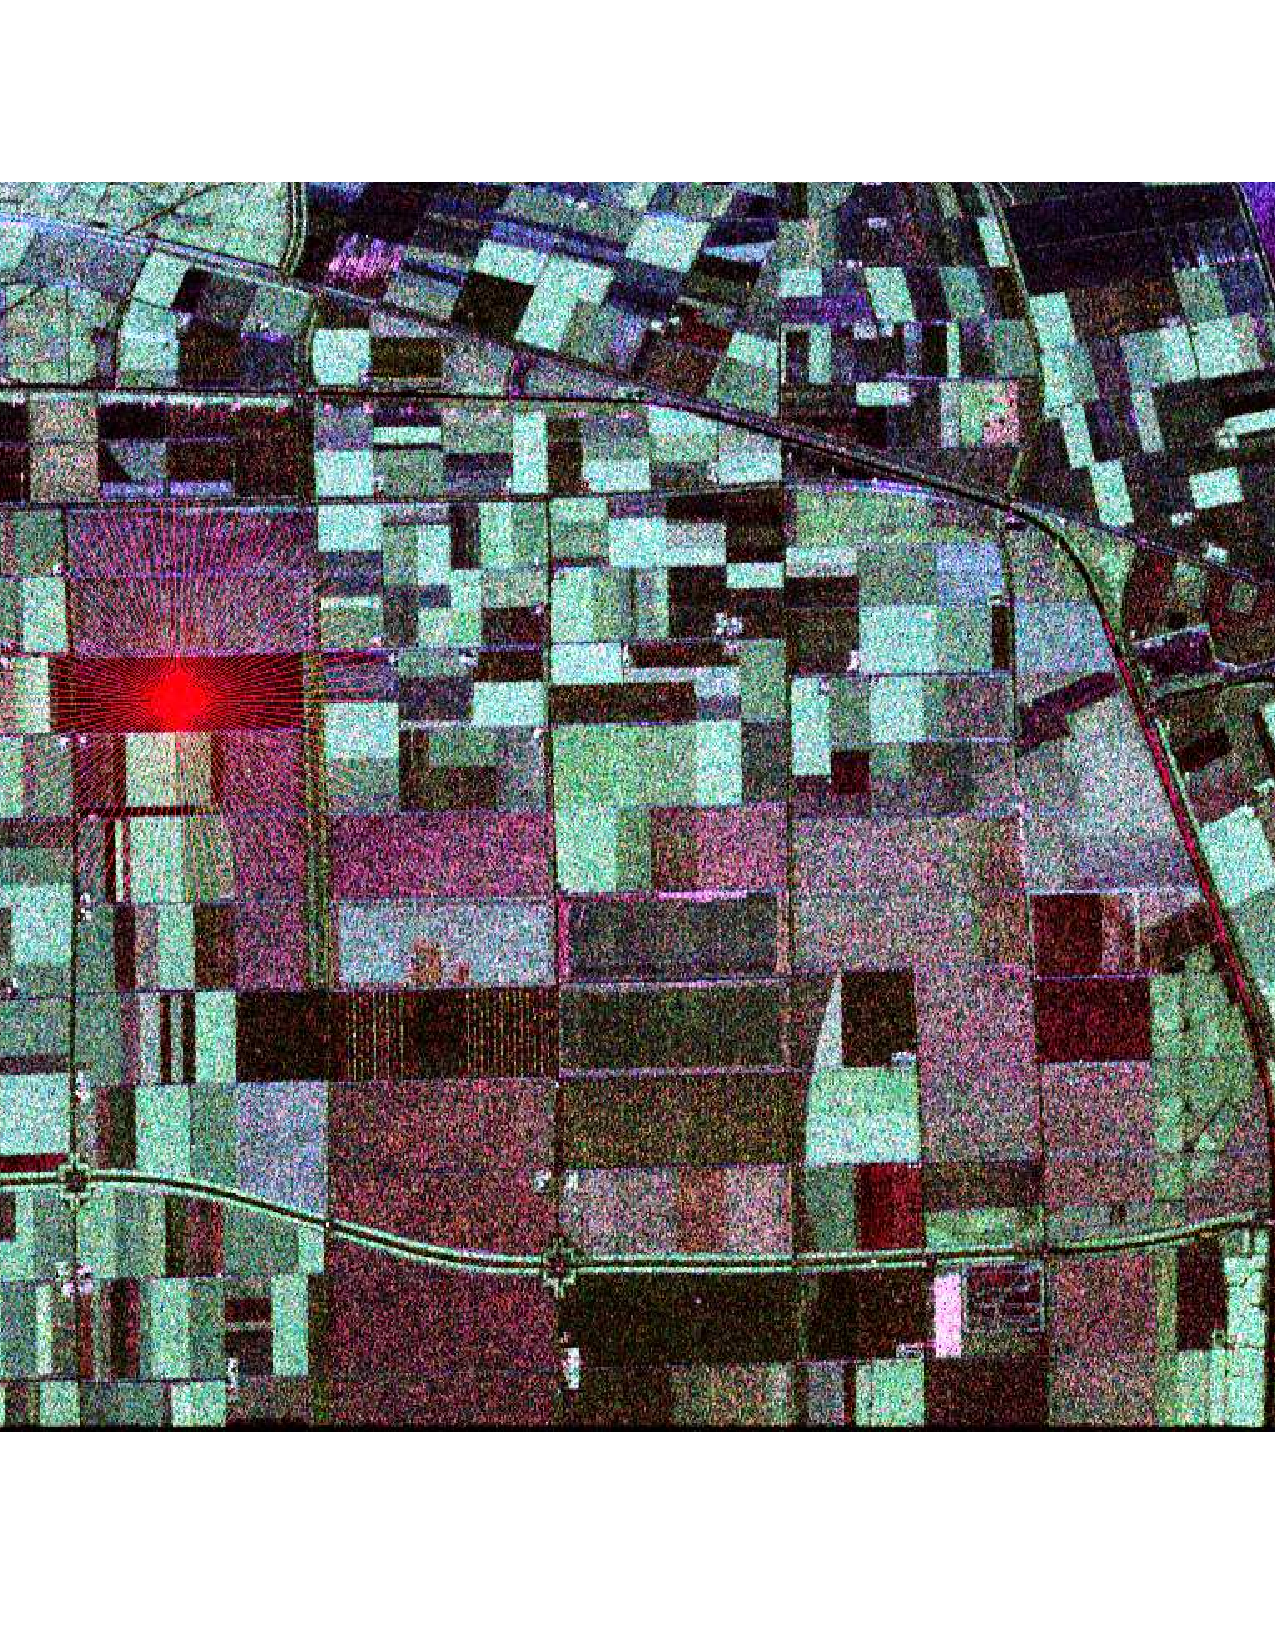
\includegraphics[scale=0.3]{flevoland_radial_4_look.pdf}
			\vspace{-1.0cm}
	\caption{Region of interest (ROI) in the image of Flavoland.}
\label{fig_01}
\end{figure}
The figures~\ref{fig_02}~\subref{fig:1a},~\subref{fig:1b} and~\subref{fig:1c} show, respectively, the edge evidence detection algorithms, applied to $(hh)$, $(hv)$ and $(vv)$ channels. 

The algorithm to detect evidence of edges worked well in the channels $(hh)$ and $(hv)$, achieving better accuracy in relation to the channel $(vv)$.  

In the canal (vv), edges that are not part of the homogeneous region of interest were detected, but are part of other edges of the image, researching the reason for this fact, we analyzed the function $l(j)$ and found that the function presents two peaks, representing possible evidence of edges, in which the largest was correctly detected. 
   \begin{figure}[!ht]
     \subfloat[Evidences in channel $(hh)$ \label{fig:1a}]{%
       %\includegraphics[width=0.2\textwidth]{example-image-a}
       \includegraphics[width=0.2\textwidth]{flevoland_hh_evid_crop_teste.pdf}       
     }
     \hfill
     \subfloat[Evidences in channel $(hv)$ \label{fig:1b}]{%
       \includegraphics[width=0.2\textwidth]{flevoland_hv_evid_crop_teste.pdf}
     }
     \\
     \centering
     \subfloat[Evidences in channel $(vv)$ \label{fig:1c}]{%
       \includegraphics[width=0.2\textwidth]{flevoland_vv_evid_crop_teste.pdf}
     }
     \caption{Edges evidences}
     \label{fig_02}
   \end{figure}

The figures~\ref{fig_03}~\subref{d} to~\subref{g} show, respectively, the fusion of evidence for the methods described in this article. In order, we list the method that shows the average of edges evidences, the method that uses the Stationary wavelet transform (SWT), the method that uses the Principal component analysis (PCA), and finally, the method based on ROC statistics.

The methods shown in the figures~\ref{fig_03}~\subref{d},~\subref{e} and~\subref{f} use all the pixels detected in the different channels. Each method weighs the pixels in the different channels with their characteristics. The average weighs the pixels in an equal manner. The (SWT) finds the coefficients of the linear combination of its wavelet bases, and the (PCA) weights the auto-vectors of the covariance matrix.

The ROC statistics method does not use all pixels of the channels, because the method is based on thresholds discarding pixels. This was observed in the figure~\ref{fig_03}~\subref{g}.

\begin{figure}[!ht]
     \subfloat[Averege fusion\label{d}]{%
       %\includegraphics[width=0.2\textwidth]{example-image-a}
       \includegraphics[width=0.2\textwidth]{flevoland_fusao_media_crop_teste.pdf}       
     }
     \hfill
     \subfloat[SWT fusion\label{e}]{%
       \includegraphics[width=0.2\textwidth]{flevoland_fusao_swt_crop_teste.pdf}
     }
     \\
     \subfloat[PCA fusion \label{f}]{%
       %\includegraphics[width=0.2\textwidth]{example-image-a}
       \includegraphics[width=0.2\textwidth]{flevoland_fusao_pca_crop_teste.pdf}       
     }
     \hfill
     \subfloat[ROC fusion\label{g}]{%
       \includegraphics[width=0.2\textwidth]{flevoland_fusao_roc_crop_teste.pdf}
     }
     \\
     %\centering
     %\subfloat[First sub-figure\label{flevoland_vv_evid_crop.pdf}]{%
     %  \includegraphics[width=0.2\textwidth]{flevoland_hv_evid_crop_teste.pdf}
     %}
     \caption{Fusion methods}
     \label{fig_03}
   \end{figure}

\section{Conclusion}\label{sec_08}
In this study, the statistical modelling approach was applied to real PolSAR data imaging. Aiming to understand the importance of information from each channel in the edge evidence fusions. The proposed algorithm was applied in intensity channels $(hh)$, $(hv)$ and $(vv)$, it was found the evidence of edges, using the maximum likelihood  method in each channel, obtaining good results. After analyzed the results obtained in the intensity channels, it was observed that the method for the edge detections worked better in the channels $(hh)$ and $(hv)$ than the channel $(vv)$, achieving a suitable accuracy.

Subsequently, the fusion of evidence of edges was performed with the methods of simple average, SWT, PCA and ROC statistics. The first three methods performed well as shown in the results. The ROC statistics method suppressed several edge points, a behaviour expected because it is a method that uses thresholds; however, when applied in a larger number of channels, its performance tends to improve. 

Based on these results, a possible way to improve them would be to increase the number of channels studied. This analysis open a path for future researches with application of different methods for edge evidence fusing.
\bibliographystyle{IEEEtran}
\bibliography{bibliografia}
\end{document}
